\documentclass[xcolor=dvipsnames,hyperref={pdfpagelabels=false}]{beamer}

\usetheme{AnnArbor}

\let\Tiny=\tiny

\newcommand{\bi}{\begin{itemize}}
\newcommand{\ei}{\end{itemize}}
\newcommand{\be}{\begin{enumerate}}
\newcommand{\ee}{\end{enumerate}}
\newcommand{\bc}{\begin{center}}
\newcommand{\ec}{\end{center}}
\newcommand{\I}{\item}
\newcommand{\f}{\frame}
\newcommand{\ft}{\frametitle}

\title{Hall D Software Overview}
\subtitle{12 GeV Software Review}
\author[Mark Ito]{Mark M.\ Ito}
\date{June 7, 2012}
\institute[JLab]{Jefferson Lab}

\begin{document}

\f{\titlepage}

\f{
\ft{Outline}
\be
\I Basic Components: Processors/Data-Formats/Databases/Management
\I Staffing
\I Computing Resource Requirements
\I Other Topics
   \bi
   \I Grid
   \I Calibration and Alignment
   \I Amplitude Analysis and GPU's
   \I Data Challenges
   \ei
\I Conclusions
\ee
}

% 1 Data/Analysis Flow Slide A variation on the above slide
% emphasizing what is done and what needs to be done. 120s (1090s)

\section{Processors}

\frame<1>[label=flow-diagram]{
\ft{Flow Diagram}
\small
\begin{columns}[c]
\begin{column}{1.0in}
\bi
\I<alert@1> boxes: processors
\I<alert@2> ovals: data formats
\I<alert@3> punch cards: databases
\ei
\end{column}
\begin{column}{3.5in}
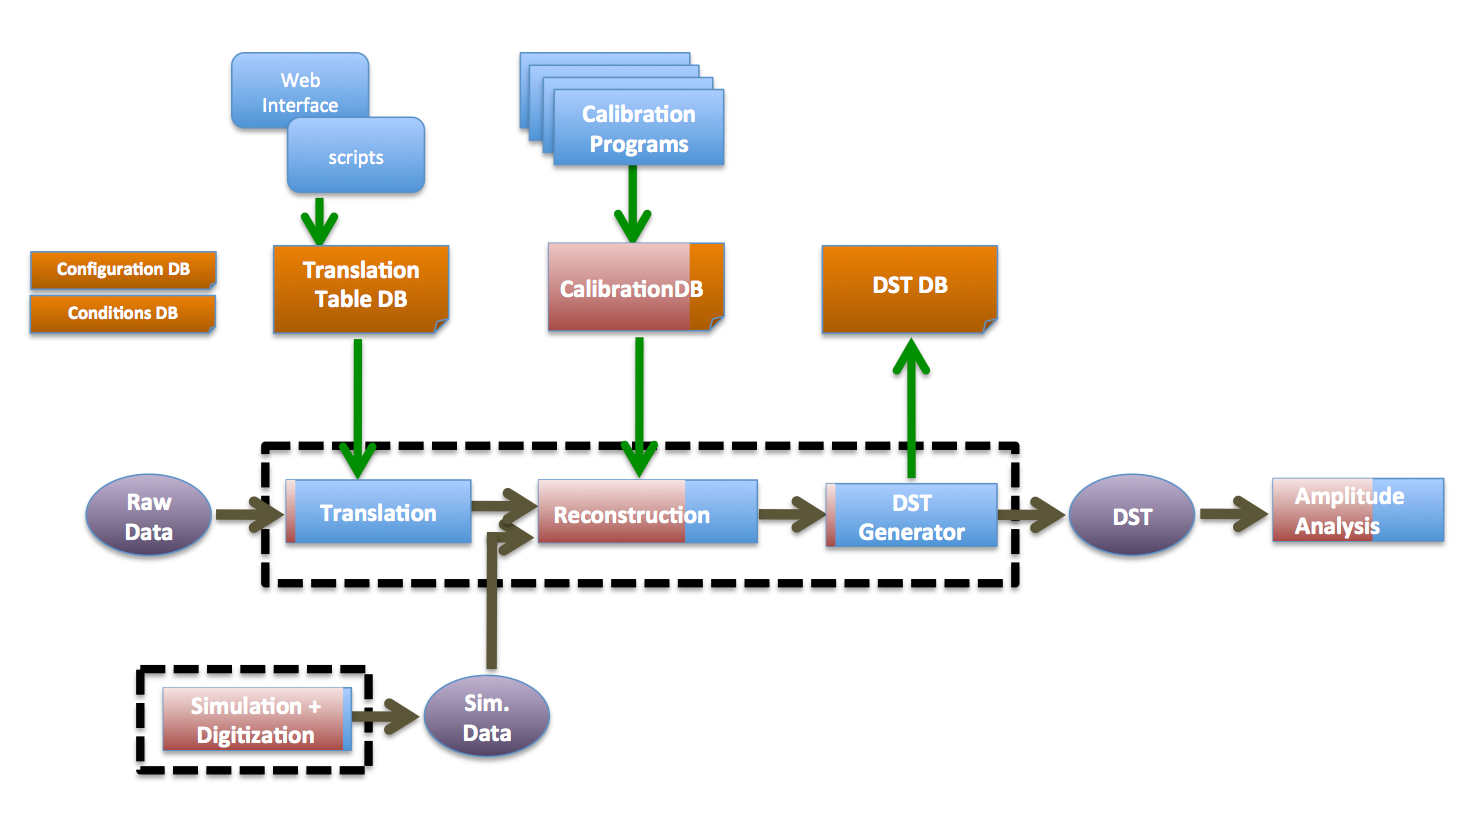
\includegraphics[width=3.5in]{DataFlow_simple.png}
\end{column}
\end{columns}
}

\subsection{Simulation}

\f{
\ft{Simulation/Digitization}
\begin{columns}[c]
\begin{column}{3.0in}
\bi
\scriptsize
\I GEANT3-based (mature)
   \bi\scriptsize
   \I Geometry defined in configuration files, not source code
      \bi\scriptsize
      \I Hall D Detector Specification (HDDS), an XML implementation
      \ei
   \I Electromagnetic background included (as accidentals)
   \I Resolution/digitization introduced in separate process (mcsmear)
   \ei
\I Geant4 Conversion
   \bi\scriptsize
   \I Started as a background task
   \I Geometry from same HDDS files as for GEANT3 implementation
   \I Hit generation: no new algorithms, re-use same core C code as before
   \ei
\ei
\end{column}
\begin{column}{1.5in}
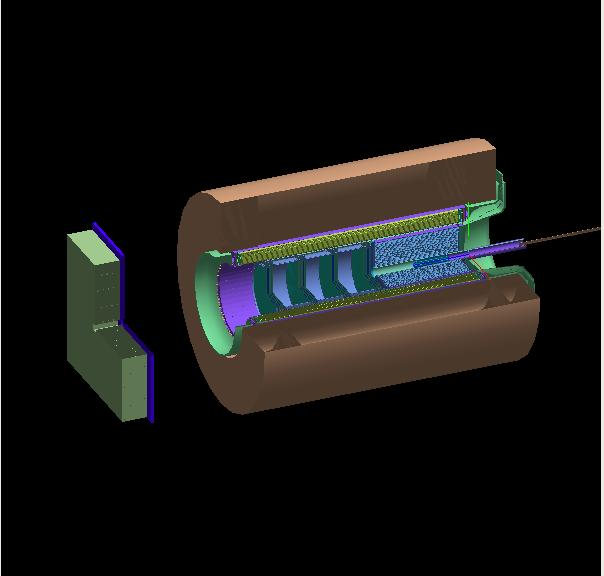
\includegraphics[width=1.5in]{cutaway.jpg}\\
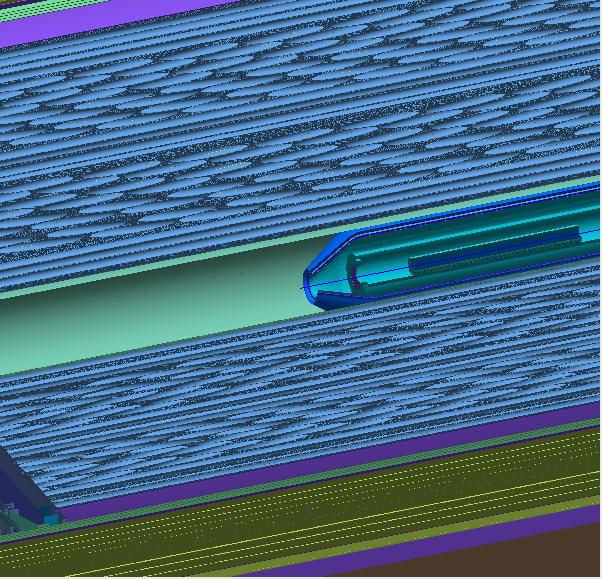
\includegraphics[width=1.5in]{cutaway_zoom.jpg}
\end{column}
\end{columns}
}

\subsection{Reconstruction}

\f{
\ft{Reconstruction}
\begin{columns}[c]
\begin{column}{2.5in}
\bi
\I Based on JANA framework (mature)
   \bi
   \I C++
   \I multi-threaded
   \I factory model
   \ei
\I Provides full feature set
\I Factories attached to framework current area of development
   \bi
   \I {\it e.~g.}, cluster finding, track fitting 
   \ei
\ei
\end{column}
\begin{column}{2.0in}
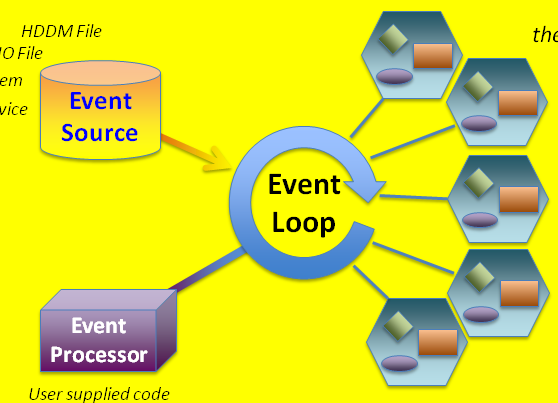
\includegraphics[width=2.0in]{jana.png}
\end{column}
\end{columns}
}

\f{
\ft{Efficiency and Resolution}
\bi
\I Reconstruction code has improved significantly over the past year
\I Remains major area of effort right now
\I Track reconstruction in a non-uniform magnetic field
   \bi
   \I curling tracks
   \I areas of reduced efficiency/resolution
   \I reconstruction speed
   \ei
\I Photon reconstruction
   \bi
   \I split-offs
   \I merged clusters
   \I effort to lower thresholds
   \I hadronic contamination
   \ei
\ei
}

\section{Data Formats}

\againframe<2>{flow-diagram}

\f{
\ft{Serialized data formats}

\begin{columns}[c]
\begin{column}{2.5in}
\bi\scriptsize
\I Raw data
   \bi\scriptsize
   \I EVIO: CEBAF Online Data Acquisition (CODA) format
   \ei
\I Simulated data
   \bi\scriptsize
   \I HDDM: Hall D Data Model, self-documenting on two levels
      \be\scriptsize
      \I data itself XML-like (compressed)
      \I each file contains complete mini-schema
      \ee
   \I support utilities for conversion
   \ei
\I DST data (reconstructed)
   \bi\scriptsize
   \I HDDM
   \I others possible
   \ei
\ei
\end{column}
\begin{column}{2.5in}
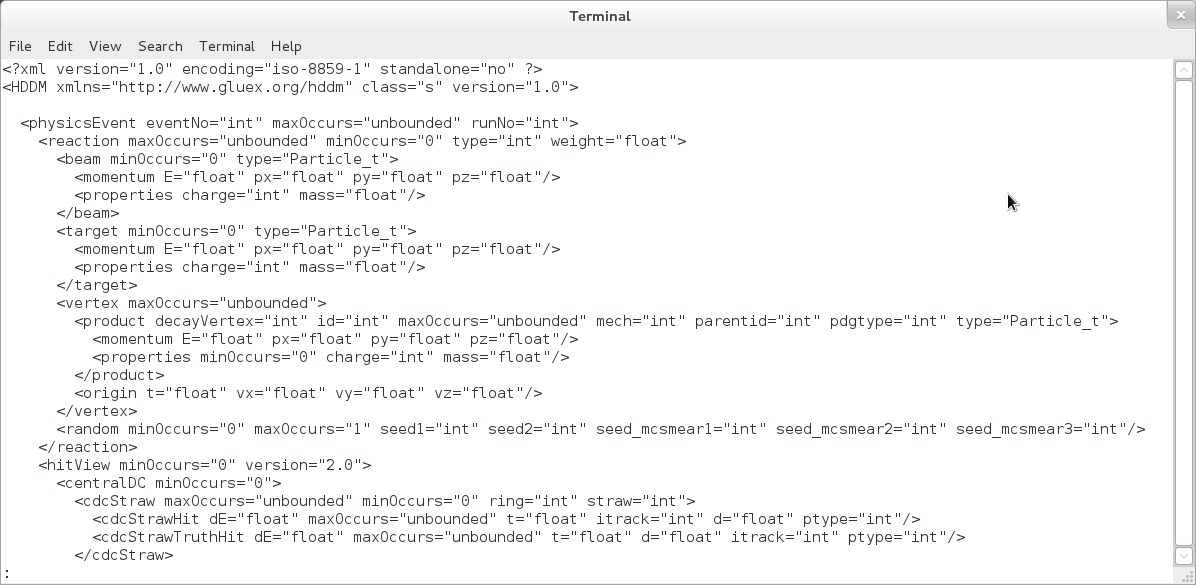
\includegraphics[width=5.0in]{hddm_template.png}//
\end{column}
\end{columns}
}

\section{Databases}

\againframe<3>{flow-diagram}

\f{
\ft{Databases}
\begin{columns}[c]
\begin{column}{2.0in}
\bi\small
\I Calibration and Conditions Database (CCDB)
   \bi\scriptsize
   \I developed by Hall D
   \I in beta testing (Hall B is using it too)
   \I put into production mid-July, 2012
   \ei
\I Other Database Applications
   \bi\scriptsize
   \I Online Conditions/Parameters
   \I Translation Tables
   \I DST
   \ei
\ei
\end{column}
\begin{column}{3.0in}
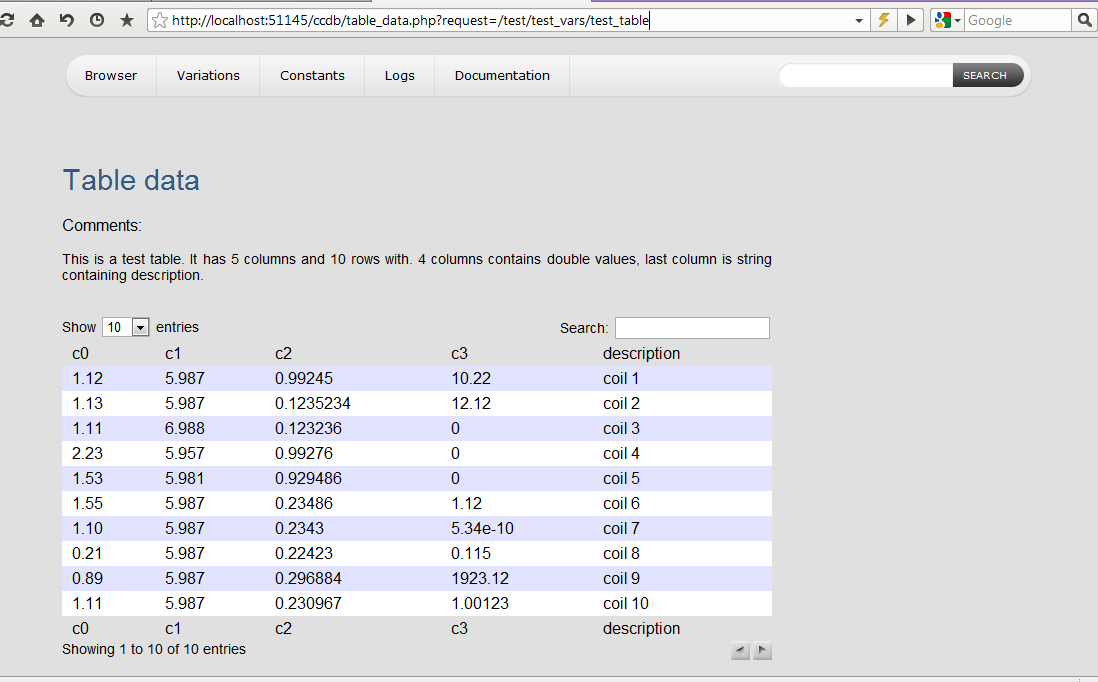
\includegraphics[width=3.0in]{CCDB_Table_data_listing.png} \\
\bi\small
\I CCDB Features:
\bi\scriptsize
   \I relational database
   \I standard look up by run
   \I hierarchical calibration type structure
   \I history kept, previous versions selectable at run time
   \I branches/private/tagged versions supported
\ei
\ei
\end{column}
\end{columns}
}

\section{Software Management}

\f{
\ft{Software Management Tools}

\bi
\I Source code version control: Subversion
\I Regular tagged releases of simulation and reconstruction software (``sim-recon''): about every 6 weeks
\I Nightly builds of sim-recon
   \bi
   \I all Lab-supported Linux flavors
   \I Doxygen documentation generated
   \ei
\I Semi-weekly tests: histograms generated, archived
   \be
   \I single-charged particles events
   \I multi-track, multi-photon events ($5\pi$) \\
\( \begin{array}{l@{}l@{}l@{}l@{}l@{}}
\gamma p \rightarrow & Xp \\
& \hookrightarrow & b^\pm_1\pi^\mp \\
&&\hookrightarrow&\omega\pi^\pm \\
&&&\hookrightarrow\pi^+\pi^-&\pi^0 \\
&&&&\hookrightarrow \gamma\gamma
\end{array} \)
   \ee
\I Mantis bug tracker for issue tracking
\ei

}

\section{Staffing}

% 2 Manpower Estimates A slide showing the broken out tasks with \%
% complete, manpower needed to complete and names of people with
% institutions that are responsible for the tasks. Conclusion that at
% least at the present, we appear to have sufficient manpower to
% complete the tasks in the time given. 120s (1210s)

\subsection{Requirements}

\f{
\ft{Staffing Requirements and Project Progress}
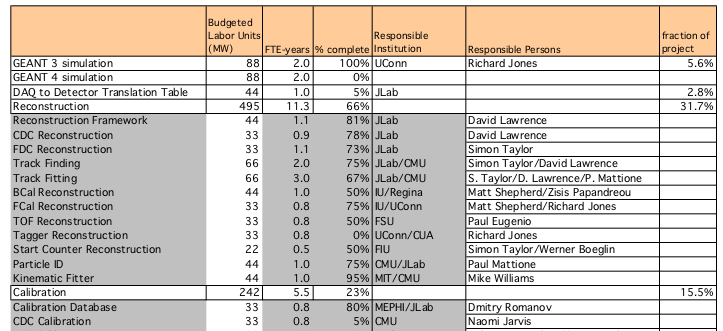
\includegraphics[width=4.75in]{OfflineComputingActivities2012Zoom.png}
\bi\small
\I Complete task list with labor estimates and fraction completed
\I Formerly tracked by 12 GeV Project Management team
\I Total effort: 38 FTE-years, complete: 51\%, remaining work: 19 FTE-years
\ei
}

\subsection{Resources}

\f{
\ft{Staffing Resources}
\bc
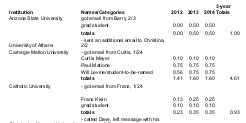
\includegraphics[width=2.8in]{manpower_survey_raw.png}
\ec
\begin{columns}[c]
\begin{column}{2.2in}
\bi\scriptsize
\I Survey of estimated staffing resources available for software infrastructure
\I Different categories weighted differently
\I Total for 2012-2014: 23 FTE-years
\I Good match with requirements, but little safety factor
\ei
\end{column}
\begin{column}{2.3in}
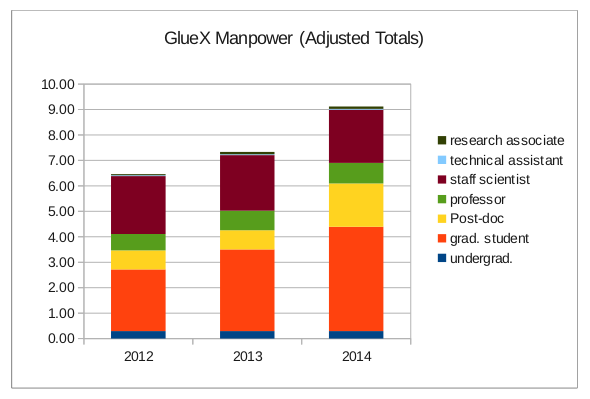
\includegraphics[width=2.3in]{manpower_survey_graphs.png}
\end{column}
\end{columns}
}

% 3 Software Management A slide showing how the Offline group is
% organized, and how it interacts with the other groups involved in
% related tasks. 60s (1270s)

%\f{
%\ft{Software Management}
%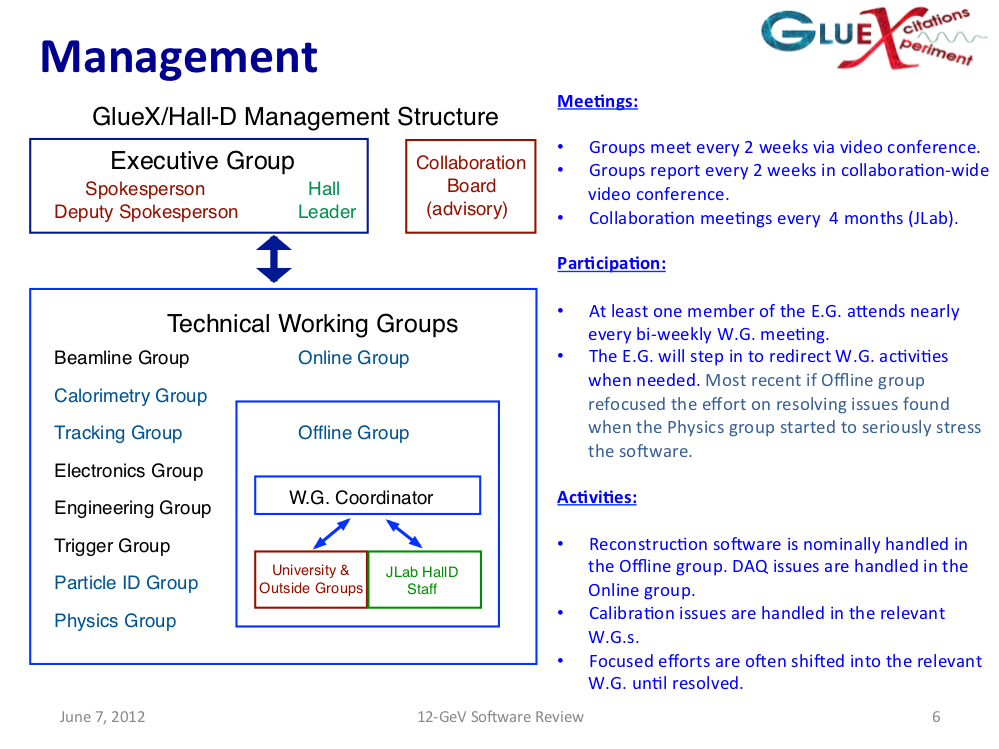
\includegraphics[height=3.0in]{org_chart_slide.png}
%}

\section{Computing Resource Requirements}

% 6 Data Analysis Model Lay out the model for analysis of GlueX
% data. Raw data on tape/disk at Jefferson Lab. DST’s produced at
% Jefferson Lab, on Tape/Disk. MiniDSTs produced at Jefferson Lab and
% then both analyzed on site and moved off site utilizing
% grid-ftp. 120s (1630s)

% 7 Simulation Lay out the model for GlueX simulation. Production both
% at Jefferson Lab and at remote sites. Simulation will produce
% MiniDSTs that will need to be moved. All other data is likely
% flushed. What are the expecte resources in outside sites? 120s
% (1760s)

\subsection{Analysis Model}

\f{
\ft{Data Analysis Model}
   \bi\small
   \I From detector to online buffer disk in Counting House
   \I Over network to Tape Library in Computer Center
   \I Reconstruction on JLab batch farm, reduction of volume by factor of 10
   \I Resulting DST data written to Tape Library: some fraction live on disk
   \I Mini-DST's (``4-vectors'') in several streams: large fraction live on disk
   \I Similiar scenario for Monte Carlo except ``raw'' Monte Carlo not kept (also at JLab)
   \I Analysis engines access this data:
      \bi
      \I JLab batch farm
      \I Individual work stations
      \I Collaborating institutions
      \I Amplitude analysis resources
      \ei
   \ei
}

% 4 Data/Compute Model A slide based on Mark’s spread sheet showing
% the way that we estimate data volumes and CPU needs. Discuss phase
% I, II and III. 120s (1390s)

\subsection{Computing Model}

\f{
\ft{Data/Computing Model}
Trigger rates:
\bi\scriptsize
\I Phase III: beam rate $10^{7}~\gamma/s$ in coherent peak
\I Full hadronic cross section $\Rightarrow$ 20~kHz trigger rate
\I Beyond Phase III: use level 3 software trigger to keep rate roughly constant
\I Start with ``monitoring farm'', upgrade to ``trigger farm'' 
\ei


Assumptions (generic):
\bi\scriptsize
\I 20 kHz off detector
\I 15 kB events
\I run 35 weeks year, 50\% running efficiency
\I 133 ms to reconstruct an event (measured)
\I 2 Monte Carlo events per data event (on average)
\I 67 ms to generate Monte Carlo events (reconstruction time comparable to data)
\I factor for multiple iterations: 2
\I Other loads:
   \bi\scriptsize
   \I calibration processing
   \I skims/mini-DST production
   \I physics analysis
   \ei
\ei

}

\subsection{Requirements}

\f{\ft{CPU and Tape Requirements}
\bc
\begin{tabular}{|l|r|r|}
\hline
Process & CPU (kCores) & Tape (PB/y)\\
\hline
Raw Data & -- & 3.2 \\
Calibration & 0.09 & 0.06 \\
Reconstruction & 1.8 & 1.3 \\
Skims/mini-DST & 0.9 & 0.6 \\
Analysis & 0.9 & -- \\
Simulation & 5.4 & 2.5 \\
\hline
Total & 9 & 8 \\
\hline
\end{tabular}
\ec

\small CPU represents amount of computing power required to keep up with average rate off detector. Sets the scale; should be viewed as a minimum requirement.
}

\f{
\ft{Another View of Requirements: Wait Time}

\bc\bf
How long do we wait for results?
\ec

Assume a 10~kCore farm, unloaded, nominal running efficiency, and one iteration only. Other assumptions the same as above.

{\small
\begin{tabular}{lrrr}
 & \bf Phase I & \bf Phase II & \bf Phase III \\
Days of running & 60 & 60 & 120 \\
Trigger rate (kHz) & 2 & 20 & 20 \\
Number of events & 5.18$\times 10^9$ & 5.18$\times 10^{10}$ & 1.04$\times 10^{11}$ \\
Reconstruction time (days) & 0.8 & 8 & 16 \\
Monte Carlo time (gen. + recon.) (days) & 2.4 & 24 & 48 \\
Reconstruction time + MC time (days) & 3.2 & 32 & 64 \\
\end{tabular}
}
}

\f{
\ft{Disk Requirements}

\bc
{\small
\begin{tabular}{p{3.0in}rr}
&\multicolumn{2}{c}{\bf Phase} \\
{\bf Data Type} & {\bf II} \scriptsize (TB) & {\bf III} \scriptsize (TB)\\
\textcolor{blue}{Calibration disk} & 62 & 124 \\
\textcolor{blue}{Coherent-peak skim DST} Reconstructed data, from coherent
  brems\-strah\-lung peak & 25 & 50 \\
\textcolor{blue}{Inclusive background simulation DST} Simulation, minimum bias & 265 & 531 \\ 
\textcolor{blue}{Individual analysis skims} Skims of data and simulation for
individual analyses, 10 analyses & 207 & 415 \\
\textcolor{blue}{Mini-DST's for amplitude analysis} 4-vectors & 7 & 15 \\ \hline
\bf Total & 567 & 1134
\end{tabular}
}
\ec

\bi
\I Disk to support analysis activities, not large-scale reconstruction/simulation
\I In addition: work/scratch/staging disk of 300~TB
\I {\bf Grand Total}: 2.0~PB 
\ei

}

% 8 Open Science Grid Discuss that GlueX is a virtual organization in
% the OSG. Some resources from outside are committed to the grid. 120s
% (1890s)

\section{Open Science Grid}

\frame{
\ft{Open Science Grid (OSG)}

\bi
\I Plan to use Grid resources to augment those at JLab
   \bi
   \I Monte Carlo generation and reconstruction (no raw data transfer)
   \I Opportunistic usage: possible to have quick turn-around on
   specific tasks
   \ei
\I Have established GlueX as a Virtual Organization (VO) with the OSG
\I Nodes from UConn have been contributed
\I Significant analysis has been performed using the grid ($3\pi$ and $5\pi$ analyses)
\I GlueX consumption has roughly matched contribution
\I Grid tools have been installed at JLab (no plan for JLab to contribute nodes)
\I Plan to use Grid Storage Resource Manager (SRM) to move data on and
off JLab site
\ei
}

\f{
\ft{Contribution and Consumption}
\begin{columns}[c]
\begin{column}{2.25in}
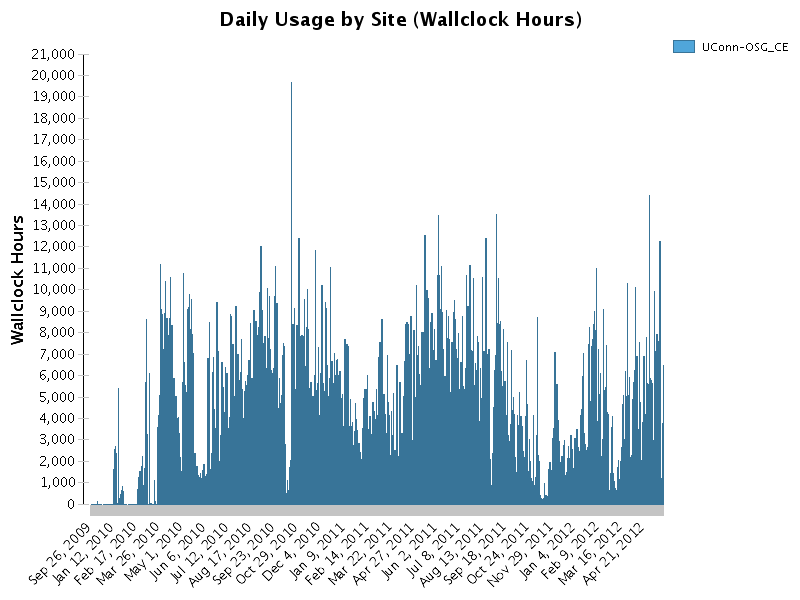
\includegraphics[width=2.25in]{osg_uconn_usage.png}\\
\bc\scriptsize OSG usage at UConn (contributed)\ec
\end{column}
\begin{column}{2.25in}
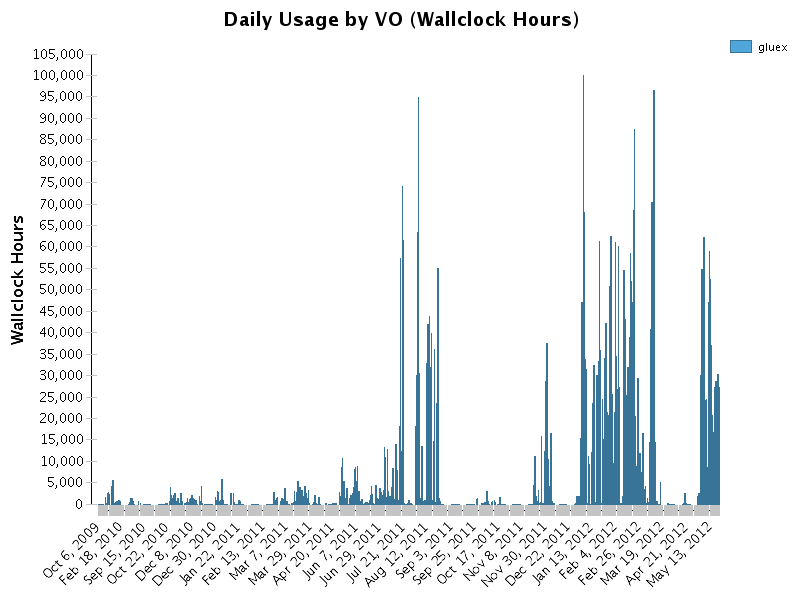
\includegraphics[width=2.25in]{osg_gluex_usage.png}
\bc\scriptsize GlueX usage on the OSG (consumed)\ec
\end{column}
\end{columns}
}

%\f{
%\ft{Expected Non-JLab Resources}
%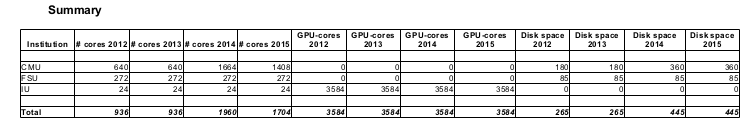
\includegraphics[width=4.5in]{ComputingResourcesZoom.png}
%\bi
%\I Have compiled info on compute farms at collaborating institutions
%\I Only UConn grid enabled
%\ei
%}

\section{Calibration and Alignment}

% 5 Calibration/Alignment What needs to be calibrated and how will it
% be done? What has been done already? pi0 calibration of the FCAL,
% CDC prototype alignment and calibration, others? Beam tests? 120s
% (1510s)

\f{
\ft{Calibration/Alignment}
\bi
\I Developing plans for calibration
   \bi
   \I Each working group tasked to list methods, data requirements, compute requirements
   \I Examples:
      \bi
      \I $\pi^0$ calibration of forward calorimeter
      \I run plan for tracking chamber alignment
      \I time walk corrections for time-of-flight using plane-to-plane information
      \ei
   \ei
\I Hardware and software have reached the point where we can turn to calibration
\I Goal: have most calibration systems available in a year
   \bi
   \I fits with detector installation time frame
   \ei
\ei
}

\section{Amplitude Analysis}

% 9 Amplitude Analysis On GPUs 60s (1950s)

\f{
\ft{Amplitude Analysis on GPU's}

\bi
\I Challenge of amplitude analysis largely met by GPU technology
\I Calculation of log likelihoods for individual events
   \bi
   \I independent for each event
   \I computationally expensive
   \I not branch intensive
   \I I/O to do computation is small
   \I results are to be summed
   \ei
\I Technique starting to be used by many experiments
\I One of leading implementations developed by GlueX collaborator: AmpTools
\I Large reduction in scale of compute task (1-2 orders of magnitude)
\I Proof-of-principle established ($3\pi$, $5\pi$)
\I Implement a user-friendly ``production'' system by Spring 2013
\ei
}

% 10 Data Challenge What sort of data challenge do we need? When? 60s
% (2000s)

\section{Data Challenges}

\f{
\ft{Data Challenges}

\bi\small
\I Simulate raw data to DST chain on a large scale
\I Need to develop job management tools
\ei

\bc\bf Data Challenge Timeline\ec
{\small
\begin{tabular}{rp{3.3in}l}
& \bf Task & \bf Date \\
1 & deploy calibration database & 2012-07-15 \\
2 & deploy translation database & 2012-09-01 \\
3 & complete raw data format specification & 2012-10-01 \\
4 & complete specification of reconstructed data format & 2012-10-15 \\
5 & data challenge: simulated raw data to DST data (one day at $10^7~\gamma/s$) & 2012-12-01 \\
6 & complete mini-DST writer & 2013-02-01 \\
7 & create mini-DST data samples from data challenge events & 2013-03-01 \\
\end{tabular}
\bc
Next step: one week's worth of data
\ec
}

}

\subsection{IT Division Collaboration}

\f{
\ft{Collaboration with IT Division's Scientific Computing Group}
\bi
\I Looking forward to continued collaborative efforts in JLab's 12 GeV era
\I Physicists want to better understand the computing resources being provided
   \bi
   \I un-steepen the learning curve for new collaborators
   \I increase efficiency in use of resources
   \ei
\I Possible areas of development:
   \bi
   \I Enhanced reporting of farm job priority/status/disposition
   \I Central support of key scientific software packages (ROOT, CERNLIB, Geant4, CLHEP)
   \ei
\ei
}

\section{Conclusions}

% 11 Summary/Conclusion Summarize where we are and where we are
% going. List of what still needs to be done? Contingencies. 60s
% (2060s)

\f{
\ft{Summary/Conclusions}
Accomplishments
\bi
\I End-to-end solution for simulation and reconstruction in hand.
   \bi
   \I realistic event generators
   \I photons and charged particles, hit-level
   \I long experience using tools
   \ei
\I Amplitude analysis capability demonstrated
   \bi
   \I GPU method developed
   \I used in $3\pi$ analysis
   \I work on $5\pi$ well along
   \ei
\ei
Work Ahead
\bi\small
\I Put calibration database into production (2012-07-01)
\I Deploy translation table database (2012-09-01)
\I Large-scale data challenge (2012-12-01)
\I Calibration software systems in full development (2013-06-01)
\I Production GPU system (2013-06-20)
\I Reconstruction quality at near-publication level (2014-03-31)
\ei
}

\section{Backup}

\f{
\bc
Backup Slides
\ec
}

\begin{frame}[fragile]
\vskip 0.5in
\hrule
\tiny
\begin{verbatim}
$Id$
\end{verbatim}
\end{frame}


\end{document}
